%
% Copyright (c) 2020 Antonio Coín Castro
%
% This work is licensed under a
% Creative Commons Attribution-ShareAlike 4.0 International License.
%
% You should have received a copy of the license along with this
% work. If not, see <http://creativecommons.org/licenses/by-sa/4.0/>.

Since as part of this bachelor's thesis we were to undertake a software development project, we prepared an estimation of the monetary costs we would incur, including the labour costs. We established an hourly price of 30€, and we divided the work in three different aspects: the theoretical study needed to understand the algorithms, the implementation itself, and the composition of the documentation describing the design and the results obtained. We also added a section for the cost of the infrastructure used to deploy our algorithms. The result of this cost estimation can be seen in Table \ref{tab:cost}.

\begin{table}[h!]
  \centering
\caption{Cost estimation for our software development project.}
\label{tab:cost}
\begin{tabular}{lrrr}
\toprule
Concept & Amount (hours) & Unitary price (€/h) & Total cost (€) \\ \midrule
Study of fuzzy theory & 20 & 30 & 600\\
Study of the MapReduce model & 15 & 30 & 450\\
Learning Scala and Spark & 40 & 30 & 1200\\
\midrule
Design of algorithms & 50 & 30 & 1500\\
Implementation of algorithms & 30 & 30 & 900\\
Testing of algorithms & 15 & 30 & 450\\
Comparative study & 5 & 30 & 150\\
\midrule
Documentation writing & 20 & 30 & 600\\
Corrections & 5 & 30 & 150\\ \midrule
Cluster (40 CPUs) & -- & -- & 10000\\
Cluster installation & -- & -- & 500\\
Cluster maintenance & -- & -- &500 \\ \midrule
Total & 200 & -- & 17000\\ \bottomrule
\end{tabular}
\end{table}

Apart from the cost estimation, we also made a temporal planning of the project, starting on September 2019 and with an expected conclusion date at the end of June 2020, as we can see in Figure \ref{fig:plan1}. The examination and holidays periods are accounted for.

\begin{figure}[h!]
\centering
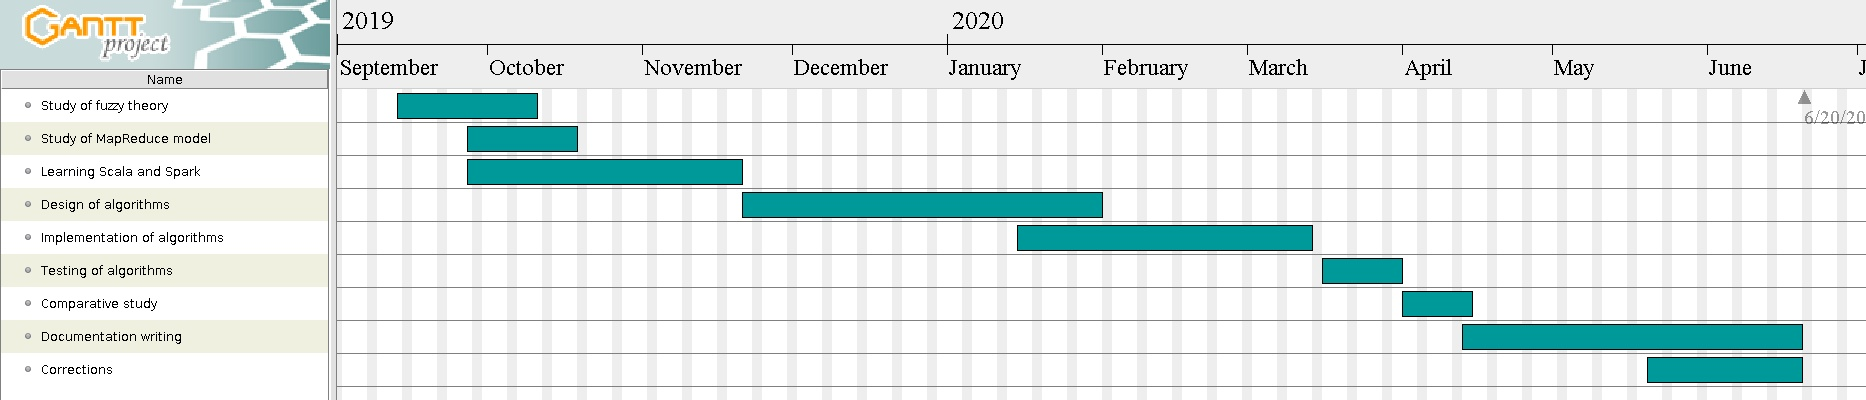
\includegraphics[width=\textwidth, height=10em]{planning1}
\caption{Temporal planning of our software development project.}
\label{fig:plan1}
\end{figure}

However, this planning turned out to be overly optimistic. We spent more time than planned in the implementation and testing of the algorithms, mainly because some unexpected difficulties arose with Spark and the way it handled some implementation details. Because of this, we had to go back and re-design some algorithms so as to avoid these obstacles. Furthermore, while conducting these tasks we entered in a worldwide crisis situation regarding the COVID-19 pandemic, so as a result the work was slower and even stopped for a short period. A more realistic estimation can be seen on Figure \ref{fig:plan2}.
\vspace{1em}
\begin{figure}[h!]
\centering
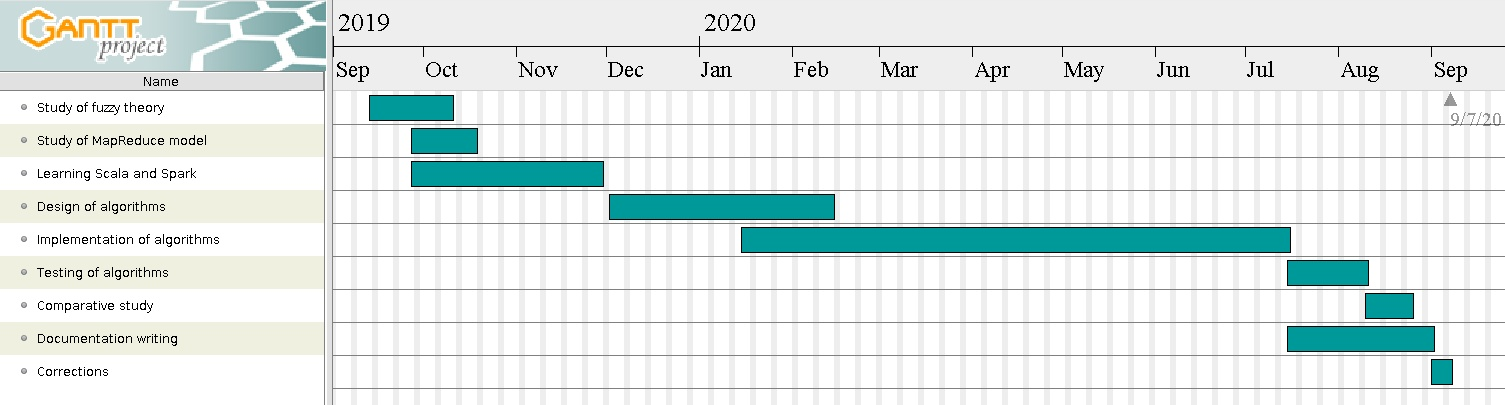
\includegraphics[width=\textwidth, height=10em]{planning2}
\caption{Realistic temporal planning of our software development project.}
\label{fig:plan2}
\end{figure}
